\documentclass{article}

% if you need to pass options to natbib, use, e.g.:
%     \PassOptionsToPackage{numbers, compress}{natbib}
% before loading neurips_2021

% ready for submission
\usepackage[preprint]{neurips_2021}

% to compile a preprint version, e.g., for submission to arXiv, add add the
% [preprint] option:
%     \usepackage[preprint]{neurips_2021}

% to compile a camera-ready version, add the [final] option, e.g.:
%     \usepackage[final]{neurips_2021}

% to avoid loading the natbib package, add option nonatbib:
%    \usepackage[nonatbib]{neurips_2021}

\usepackage[utf8]{inputenc} % allow utf-8 input
\usepackage[T1]{fontenc}    % use 8-bit T1 fonts
\usepackage[colorlinks=true]{hyperref}       % hyperlinks
\usepackage{url}            % simple URL typesetting
\usepackage{booktabs}       % professional-quality tables
\usepackage{amsfonts}       % blackboard math symbols
\usepackage{nicefrac}       % compact symbols for 1/2, etc.
\usepackage{microtype}      % microtypography
\usepackage{xcolor}         % colors
\usepackage{graphicx}

\title{Predicting Case Fatality Rate for COVID-19 from outside air temperature}

% The \author macro works with any number of authors. There are two commands
% used to separate the names and addresses of multiple authors: \And and \AND.
%
% Using \And between authors leaves it to LaTeX to determine where to break the
% lines. Using \AND forces a line break at that point. So, if LaTeX puts 3 of 4
% authors names on the first line, and the last on the second line, try using
% \AND instead of \And before the third author name.

\author{%
  Benedikt Hopf\\
  Matrikelnummer 4243889\\
  \texttt{benedikt.hopf@student.uni-tuebingen.de} \\
}

\begin{document}

\maketitle

\begin{abstract}

  In this project I use \href{https://www.arcgis.com/sharing/rest/content/items/f10774f1c63e40168479a1feb6c7ca74/data}{German COVID-19 data} from the \href{https://www.rki.de/DE/Home/homepage_node.html}{RKI (Robert Koch Institut)} together with \href{https://opendata.dwd.de/climate_environment/CDC/observations_germany/climate/hourly/air_temperature/}{German Weather Data}, provided by the \href{https://www.dwd.de/DE/Home/home_node.html}{Deutscher Wetterdienst (German Weather Service)}, to predict the COVID-19 case fatality rate using outside air temperature and time since outbreak. I use a simple custom model to recreate the actual numbers and show, that COVID-19 in Germany might have been much worse, had the breakout been a couple months earlier.

\end{abstract}

\section{Introduction}
\label{sec:introduction}

The pandemic caused by SARS-CoV-2 and the accompanying disease COVID-19 are clearly one of if not the largest worldwide crisis since the second world war. The virus originated in Wuhan, China in late 2019 and then quickly spread over the entrire world, reaching Germany on January 2nd 2020 for the first time. The first wave then followed in March 2020~\cite{rki_2022}.  

Obviously the development of a pandemic depends on many factors, but a recurring theme seems to be, that cases and case fatality rates are lower in summer, most likely due to higher temperatures. Therefore people spend more time outside where aerosole transmission is harder, and as such fewer people get infected. And the ones that do do not get quite as sick, as the dose of virus the recieved was smaller. This is a similar effect as the wearing of masks and as such very resonable.
% TODO: add citation for this claim

So in this work we will see, how well case fatality rate can be predicted from outside temperature and the time passed since the first outbreak, since this also seems to lower case fatality rate. We will not look at the number of infections, since this is highly dependent on political measures like lockdowns and as such very hard to model. 

\section{About the data}

For this task two sources of data have been used: For one this is the official German COVID-19~\cite{rki_2022} data as probided by the Robert Koch Institute, which is the German autority that is officially responsible for tracking the pandemic, backed by the German Bundesministerium für Gesundheit (federal Ministry for health). The temperature data~\cite{dwd_2022} for Germany has been retrieved from the Deutscher Wetterdienst (German weather service), which is the official autority for weather in Germany, backed by the German Bundesministerium für Digitales und Verkehr (federak Ministry of digital matters and health). 

Looking at the two datasets (case fatality rate and air temperature) next to each other it is immediately obvious, that there seems to be a negative correlytion between them. High temperatures go with lower case fatality rates and vice versa. A possible explanation for this has already been given in section \ref{sec:introduction}. Another thing to note, is that the case fatality rate is generally decreasing, which is likely due to medical advances and increasing immunity in the population.

\section{Modelling case fatality rate}
\label{sec:modelling}

This section will discuss the model choice and provide some plots, that demonstrate model performance.

\subsection{The model}

As the model for this problem, a multiplicative model of an exponential and a sigmoid as been chosen: \begin{equation}
  a \cdot e^{b \cdot (t - \Delta)} \cdot \sigma \left( c \cdot (\vartheta - d) \right) \in \mathbb{R}
\end{equation} where \begin{itemize}
  \item $t$ is the time since the first case in days.
  \item $\vartheta$ is the outside air temperature in $^\circ C$.
  \item $a$ is a multiplicative scaling factor in $\frac{deaths}{cases}$.
  \item $b$ is the rate of decay of the case fatality rate due to time, given in $\frac{1}{days}$.
  \item $c$ is a multiplicative factor for the influence of temperature, given in $\frac{1}{^\circ C}$.
  \item $d$ is an offset for temperature, given in $^\circ C$.
  \item $\sigma$, refers to the logistic sigmoid $\sigma(x) = \frac{1}{1 + e^{-x}}$.
  \item $\Delta$ is the day of the peak of the case fatality rate during the first wave.
\end{itemize}

Note, that $\Delta$ is mathematically unnecessary as it can be completely absorbed in $a$, and only serves to \textit{center} the at a fixed location and thus make the parameters more interpretable. $t$ and $\vartheta$ are the inputs, $a, b, c, d$ are learned and $\Delta$ is fixed.

This model has several advantages, compared to a simple linear model like \begin{equation}
  a \cdot t + b \cdot \vartheta + c.
\end{equation}
These advantagees are in the range of the inputs and the result. Case fatality rate is a metric that cannot become smaller than 0, which a linear model could. 

Also the reason to include the temperature is, that it is assumed to be a measure of how much time people spend outside. This is a metric, that can attain values in $[0, 1]$ and neither more nor less. When it gets warm in summer at maximum all people can be outside at all times and never more. The same hold on the other side in winter. 

Time is included, as it can measure medical progress, which makes sense to be quite quick in the beginning and then becoming slower over time, as there are less undiscovered easy improvements. So an exponential fits that shape.

Finally a multiplicative model makes more sense than an additive on, since the assumption is, that good enough medical advancements can eventually counteract temperature variations completely and high temperatures make, that medical help is not as necessary, which cannot be represented by a additive model. In a multiplicative model one of the factors becoming (close to) 0, results in the entire output being (close to) 0.

\subsection{Training and basic evaluation}

The model was then trained using \texttt{scipy.optimize}'s \texttt{minimize} routine and the \textit{Nelder-Mead} method. The resulting fit can be seen in Figure \ref{fig:prediction}. One can see, that prediction oscillates strongly, since also temperatures are oscillating a lot. For this reason another line has been plottend, that is a 14 day average of the prediction. In general the prediction follows the acual case fatality rate pretty well.

\begin{figure}[hbt!]
  \begin{center}
    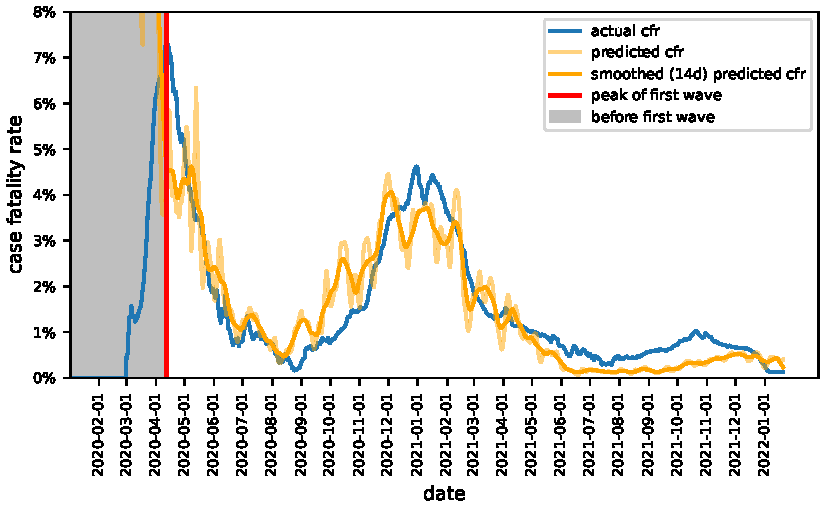
\includegraphics{../fig/prediction.pdf}
    \caption{Actual case fatality rate and predicted case fatality rate plotted againt time. The smoothed line has been created by averaging over 14 days.}
    \label{fig:prediction}
  \end{center}
\end{figure}

Since the model is designed in such a way, that it cannot capture the beginning of a pandemic (as case fatality rate most be monotonic as a function of time), the model has only been trained starting from the peak of the first wave and should only be evaluated from there. The time before that is shown in the plot, but marked as before the beginning. 

Another way to evaluate the model and see, where it has some problems, is to plot a heatmap of case fatality rate given temperature and date. This map cannot be completely covered by actual data, since some values are never attained (like $30^\circ C$ in January). Then these parts are then filled with predictions, where the goal is, that the difference between actual values and predictions are hard to distinguish. This result can be seen in figure \ref{fig:heatmap}. One can see, that the model does quite well, however different temperatures within one month are hardly different in reality, which the model does not predict quite as much. This makes sense, since for example even a relatively warm winter day will not attract as many people outside as a cold spring day (with the same temperatuer) might, since it is simply not as nice outside.

\begin{figure}[hbt!]
  \begin{center}
    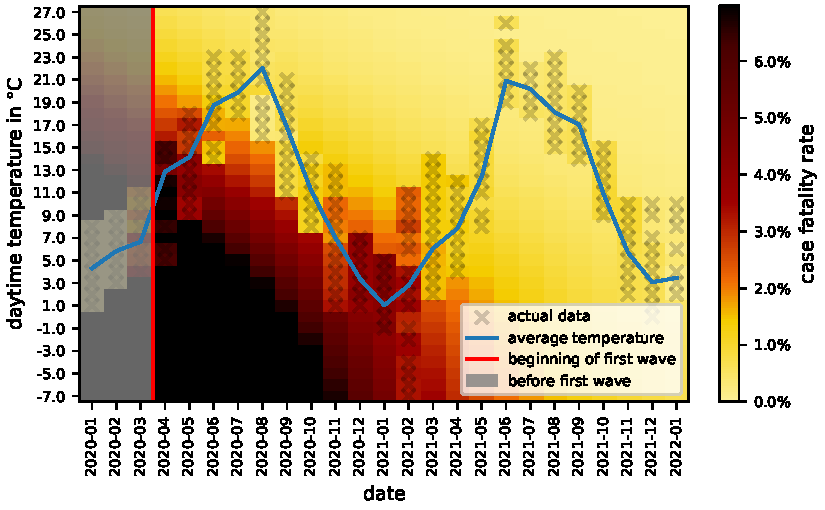
\includegraphics{../fig/heatmap.pdf}
    \caption{Heatmap of case fatality rate. x and y axis denote date and temperature respectively. The color of each square denotes the average case fatality rate under these circumstances. The actual attained values are plotted on to and marked with a faint cross. Everything that is not marked with a cross is an estimate by the model. The goal here is to be able to 'hide' the actual data well in the prediction, which is achieved reasonably well.}
    \label{fig:heatmap}
  \end{center}
\end{figure}

\section{Scenario simulation}

Now, that we have seen, that the model works decently well on data, that we know the right answer to, we can start with the actual interesting part of predicting, what would have happende, had the pandemic arrived in Germany at a different time. 

A scenario like this has been calculated for every month for one year before the actual outbreak and is shown in figure \ref{fig:cfr_timeseries}. One can see, that most curves peak much higher, which makes sense, since the actual pandemic was relatively quickly slowed down by the coming summer, which helped a lot at a time, where the pandemic was still very young. A more qualitative statement about that can be seen in figure \ref{fig:max_mean_cfr}. 

\begin{figure}[hbt!]
  \begin{center}
    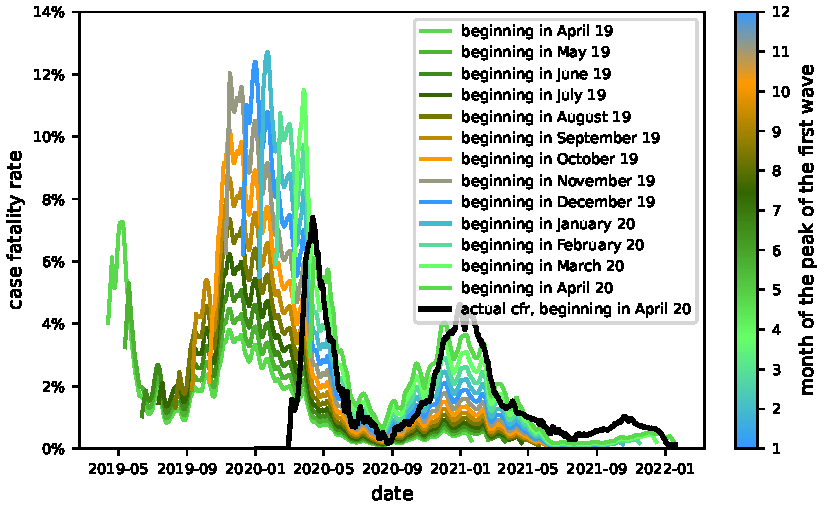
\includegraphics{../fig/CfrTimeseries.pdf}
    \caption{Predicted scenarios for outbreak (relative to the peak of the actual first wave) up to one year before April 2020. The actual case fatality rate is shown in black. The predictions colorcoded by the season, their beginning falls into.}
    \label{fig:cfr_timeseries}
  \end{center}
\end{figure}

\begin{figure}[hbt!]
  \begin{center}
    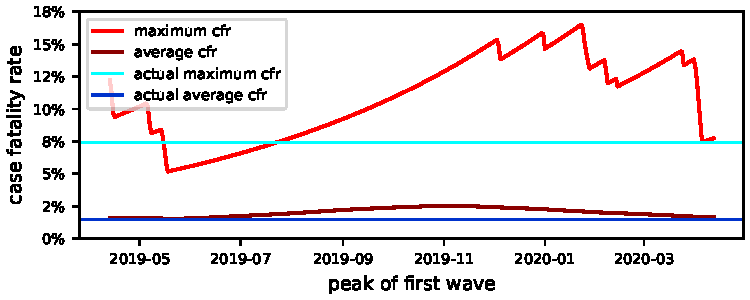
\includegraphics{../fig/MaxMeanCfr.pdf}
    \caption{Maximum and mean case fatality rate as a function of the time of outbereak}
    \label{fig:max_mean_cfr}
  \end{center}
\end{figure}

\section{Caveats}
\label{sec:caveats}

Obviously a pandemic is a very complex matter and cannot be described sufficiently well by just time since outbreak and outside air temperature. There are many other factors, that play a role in that, such as the wearing of facemasks, vaccination (which is somewhat accounted for in the decay over time) and the arising of different variants, such as the recent Omicron variant. As such these prediced scenarios might be far of. Also the case fatality rate should not be confused with the number of deaths, since a higher number of deaths would lead to stronger political reaction, which in turn would reduce the number of new infections. 

On the other hand the models predictions on past data are quite reasonable and there exists a convincing explanation for why things get prediced as they do as well as why the model is setup as it is (see sections \ref{sec:introduction} and \ref{sec:modelling}).

\section{Conclusion}

Concluding one can say, that it is reasonably possible to predict case fatality rate from air temperature and time since outbreak, using a relatively simple and explainable model (section \ref{sec:modelling}). However, these predictions are by no means perfect or guaranteed to be correct, as discussed in section \ref{sec:caveats}, since there are a vast number of factors playing into a pandemic, such as political decisions. 

Keeping in mind these caveats, the model was then used to predict, the average and maximum case fatality rates, if the pandemic had had its outbreak at an earlier time. Doing so it is quite obvious, that we have been somewhat lucky, in terms of the time of outbreak, since most scenarios would have resulted in higher maximum case fatality rates and almost all of them in higher average case fatality rates. 

% TODO: push to github and link

\bibliographystyle{plain}
\bibliography{citations}


\end{document}
